\documentclass[12pt]{article}
\usepackage[utf8]{inputenc}
\usepackage[english]{babel}
\usepackage[dotinlabels]{titletoc}
\usepackage{mathptmx}
\usepackage{amsmath, amssymb}
\usepackage{geometry, titlesec, setspace, enumitem}
\usepackage{xcolor, graphicx, caption, subcaption}
\usepackage{hyperref, natbib}
\usepackage{tabularx}
\usepackage{lipsum}
\usepackage{lmodern}
% Journals
\newcommand{\aap}{A\&A}
\newcommand{\aj}{AJ}
\newcommand{\apj}{ApJ}
\newcommand{\apjl}{ApJL}
\newcommand{\araa}{ARA\&A}
\newcommand{\mnras}{MNRAS}
\newcommand{\nat}{Nature}
\newcommand{\pasa}{PASA}
\newcommand{\pasp}{PASP}
\newcommand{\physrep}{PhR}
\newcommand{\prd}{PhRvD}
\newcommand{\rpph}{RPPh}

% Page formatting
\geometry{
	left=1.25in,
	right=1.25in,
	top=1in,
	bottom=1in}
\hypersetup{
	colorlinks=true,
	citecolor=blue,
	filecolor=blue,
	linkcolor=blue,
	urlcolor=blue
}
\setlength{\footnotesep}{10pt}
\setlist{noitemsep}

% Fixing titlesec and hyperref interaction
\makeatletter
\def\ttl@useclass#1#2{%
\@ifstar
{\ttl@labeltrue\@dblarg{#1{#2}}}
{\ttl@labeltrue\@dblarg{#1{#2}}}}
\makeatother

% Image setup
\graphicspath{{images/}}
\captionsetup[figure]{labelfont={bf}, font={small, stretch=1.3}, name={Figure}, labelsep=period}

% Section and subsection headings
\titleformat{\section}{\normalsize\bfseries\centering}{}{0em}{}
\titleformat{\subsection}{\normalsize\itshape\centering}{}{0.75em}{}
\newcommand{\nocontentsline}[3]{}
\newcommand{\tocless}[2]{\bgroup\let\addcontentsline=\nocontentsline#1{#2}\egroup}
\renewcommand{\contentsname}{Table of Contents}
\renewcommand{\abstractname}{{\normalsize\bfseries\centering{Abstract}}}
\renewcommand{\bibsection}{}

% For figures
\makeatletter
\setlength{\@fptop}{0pt plus 1fil}
\setlength{\@fpbot}{0pt plus 1fil}
\makeatother

% For formatting text and math
\let\vec\mathbf
\newcommand{\code}[1]{{\fontfamily{qcr}\selectfont#1}}
\newcommand{\red}[1]{\textcolor{red}{#1}}
\newcommand{\note}[1]{\textcolor{violet}{#1}}

% Special commands
\newcommand{\HI}{H\,\textsc{i}}
\newcommand{\OI}{O\,\textsc{i}}
\newcommand{\heraqm}{\code{hera\textunderscore qm}}
\newcommand{\herapspec}{\code{hera\textunderscore pspec}}
\newcommand{\herasim}{\code{hera\textunderscore sim}}
\newcommand{\pyuvdata}{\code{pyuvdata}}



\begin{document}
\doublespacing
\thispagestyle{empty}
\newpage
\pagenumbering{arabic}

\begin{center}
	{\Large \textbf{Cross-Correlation between the Epoch of Reionization Intensity Mapping Experiments, HERA and SPHEREx}} \\
	[0.15\textheight]

	Prepared for: \\
	Daniel Jacobs, Adam Beardsley, \& Judd Bowman \\
	Arizona State University \\
	School of Earth and Space Exploration \\[0.15\textheight]

	Prepared By: \\
	Tyler Cox \\
	Arizona State University \\
	School of Earth and Space Exploration \\
	Astrophysics Senior Thesis \\
	December 10$^{\textrm{th}}$ 2019 \\
	[0.15\textheight]

\end{center}
\thispagestyle{empty}

\clearpage
\pagenumbering{roman}

\begin{center}
	\textbf{Abstract}
\end{center}

asdf


\begingroup
\hypersetup{
	citecolor=DarkBlue,
	filecolor=black,
	linkcolor=black,
	urlcolor=DarkBlue
}
\renewcommand{\thesection}{\Roman{section}}
\tableofcontents
\listoffigures
\endgroup

\newpage

	\begin{center}
		\textbf{Acknowledgements}
	\end{center}

		First and foremost, I would like to thank the research advisors I've had since
I've joined the Low-Frequency Cosmology Lab (in no particular order), Adam Beardsley,
Judd Bowman, and Danny Jacobs. I am incredibly appreciative of your mentorship,
advice, and support.

Thank you to my third committee member, Alex Van Engelen, for enthusiastically
agreeing to sit on my committee despite the late notice.

I would also like to thank my friends, fellow students, and colleagues
who have made my time at ASU as enjoyable as it has been. In particular, I would like to
thank Shane Bechtel, Lily Whitler, and Samuel Nigh for their support and friendship.
I would also like to thank Lindsay Berkhout, Mrudula Gopalkrishna, Matt Kolopanis,
Steven Murray, and all of the members of the Low-Frequency Cosmology Lab.

Finally, I would like to send a heartfelt thank you to my parents and sister
for their constant love and encouragement.

\clearpage


\pagenumbering{arabic}


%----------------------------------%
%						Introduction					 %
%----------------------------------%

\tocless\section{\hypertarget{sec:introduction}{1.\hspace{0.75em}Introduction}}
\addcontentsline{toc}{section}{1.\hspace{0.75em}Introduction}

	\tocless\subsection{\hypertarget{subsec:universe}{1.1.\hspace{0.75em}The Early Universe}}
	\addcontentsline{toc}{subsection}{1.1.\hspace{0.75em}The Early Universe}


		Immediately following the Big Bang, the Universe was primarily composed of a hot plasma of fundamental particles. In its early state, it was  too hot and dense to form the atoms that form the complex structures that we observe today. Photons that were emitted during this early period scattered off free particles, leaving the Universe opaque to electromagnetic radiation. This lasted until roughly 400,000 years after the Big Bang, at which time the Universe had expanded and cooled sufficiently for electrons to bind to atomic nuclei forming the first atoms of hydrogen and helium. Once formed, photons were able to freely propagate through the intergalactic medium (IGM). Today, we observe this cosmic microwave background radiation (CMB).

\begin{figure}[th]
	\centering
	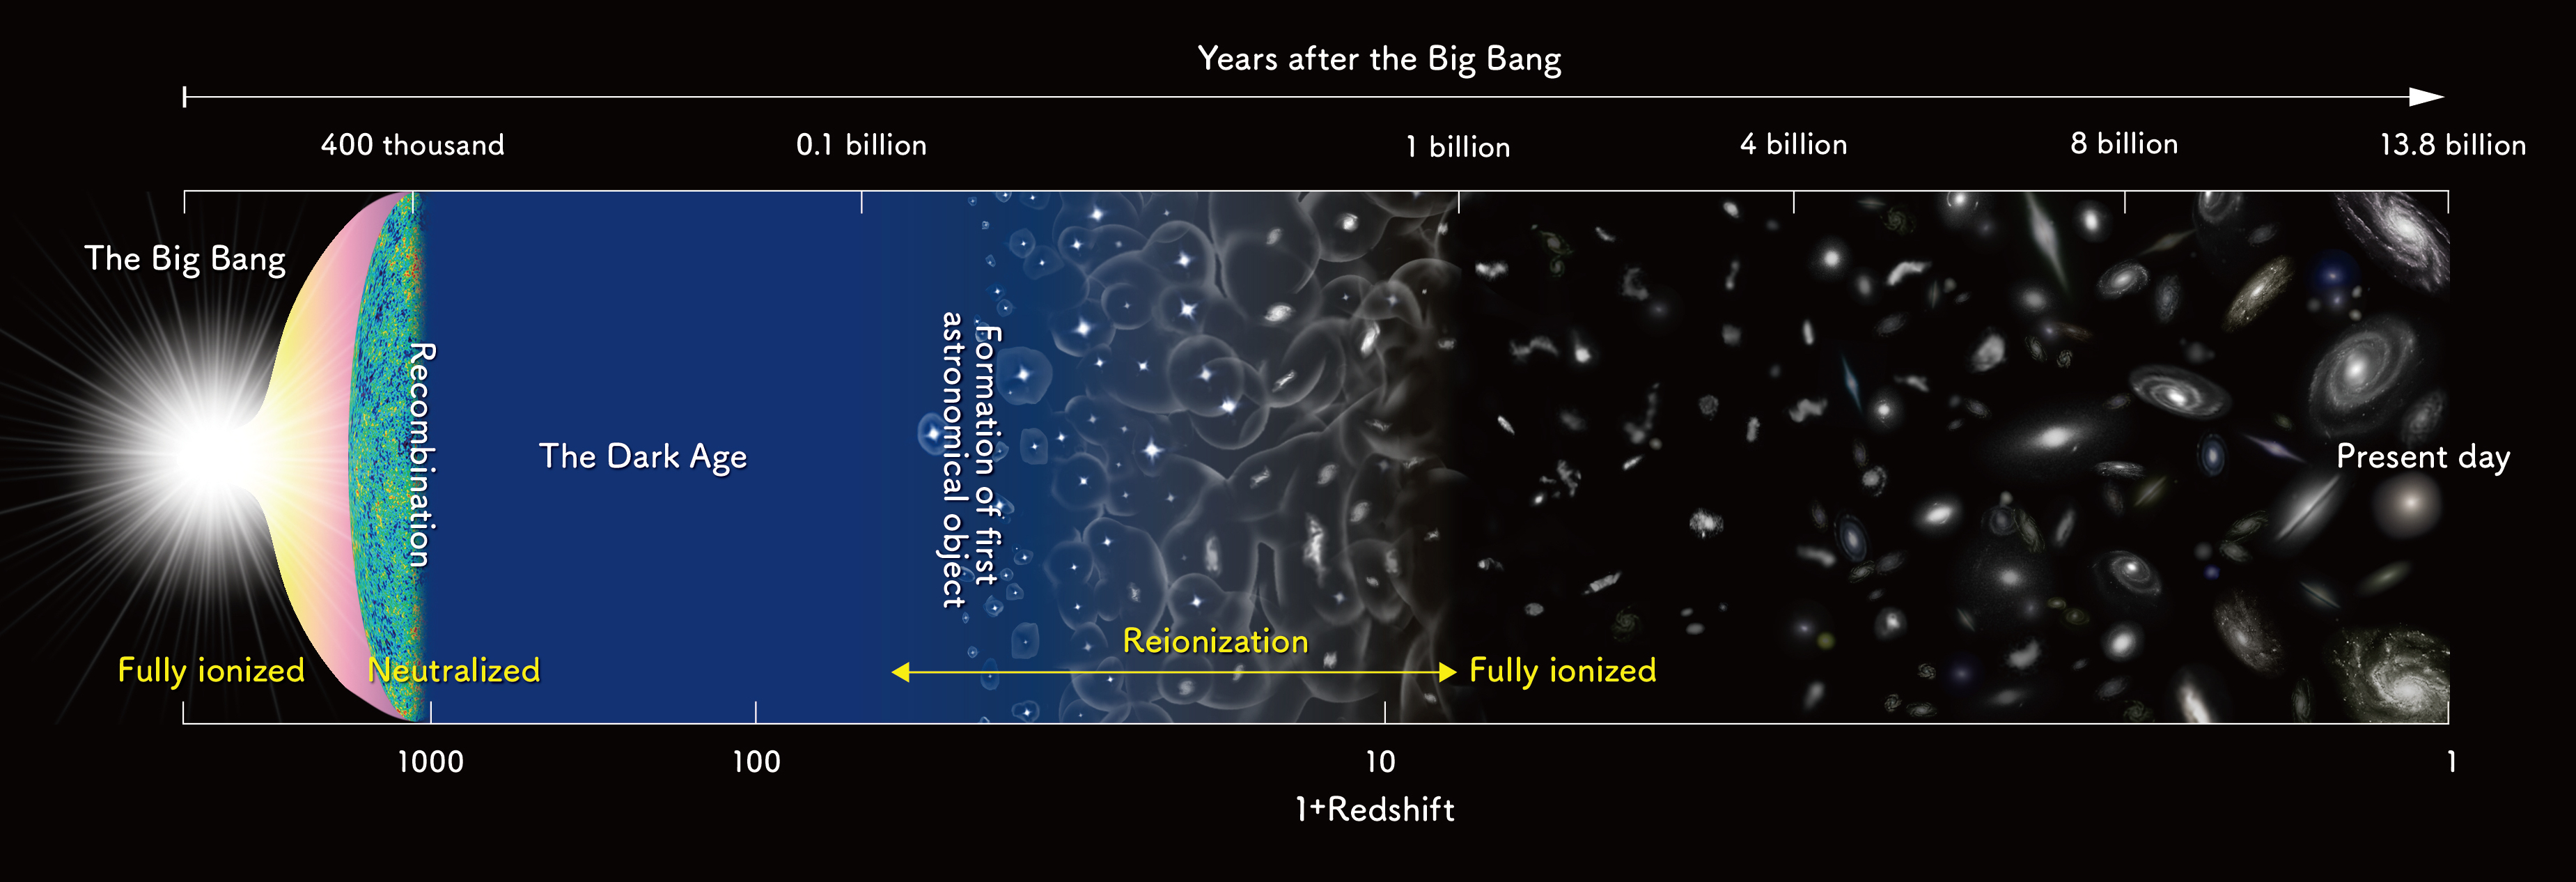
\includegraphics[width=1.0\textwidth]{intro/reionization.png}
	\caption[Epoch of Reionization Timeline]{Timeline of the history of the universe from its formation (left) to present day (right).}
	\label{fig:timeline}
\end{figure}

Following this recombination of matter, the universe was largely neutral and stationary.
Stars had not yet formed and the only emission detectable from this period originated
from neutral hydrogen. This period, called the Cosmic Dark Ages, lasted until roughly a few hundred millions after the Big Bang,
at which time the first luminous sources came into existence. Emitting ultraviolet (UV)
radiation, these first stars and galaxies began ionizing the neutral gas around them.
This period of time between the emergence of the first luminous sources and the
ionization of the neutral gas between them, named the Epoch of Reionization (EoR),
is believed to have lasted until around a billion years after the Big Bang.

Today, galaxies . Studying the EoR provides us the opportunity to establish a
bridge between the CMB and the structures we observe today, as well as provide
insight to what the first luminous objects were like and how they formed.


	\tocless\subsection{\hypertarget{subsec:eor}{1.2.\hspace{0.75em}The Epoch of Reionization}}
	\addcontentsline{toc}{subsection}{1.2.\hspace{0.75em}The Epoch of Reionization}

		

\begin{figure}[th]
	\centering
	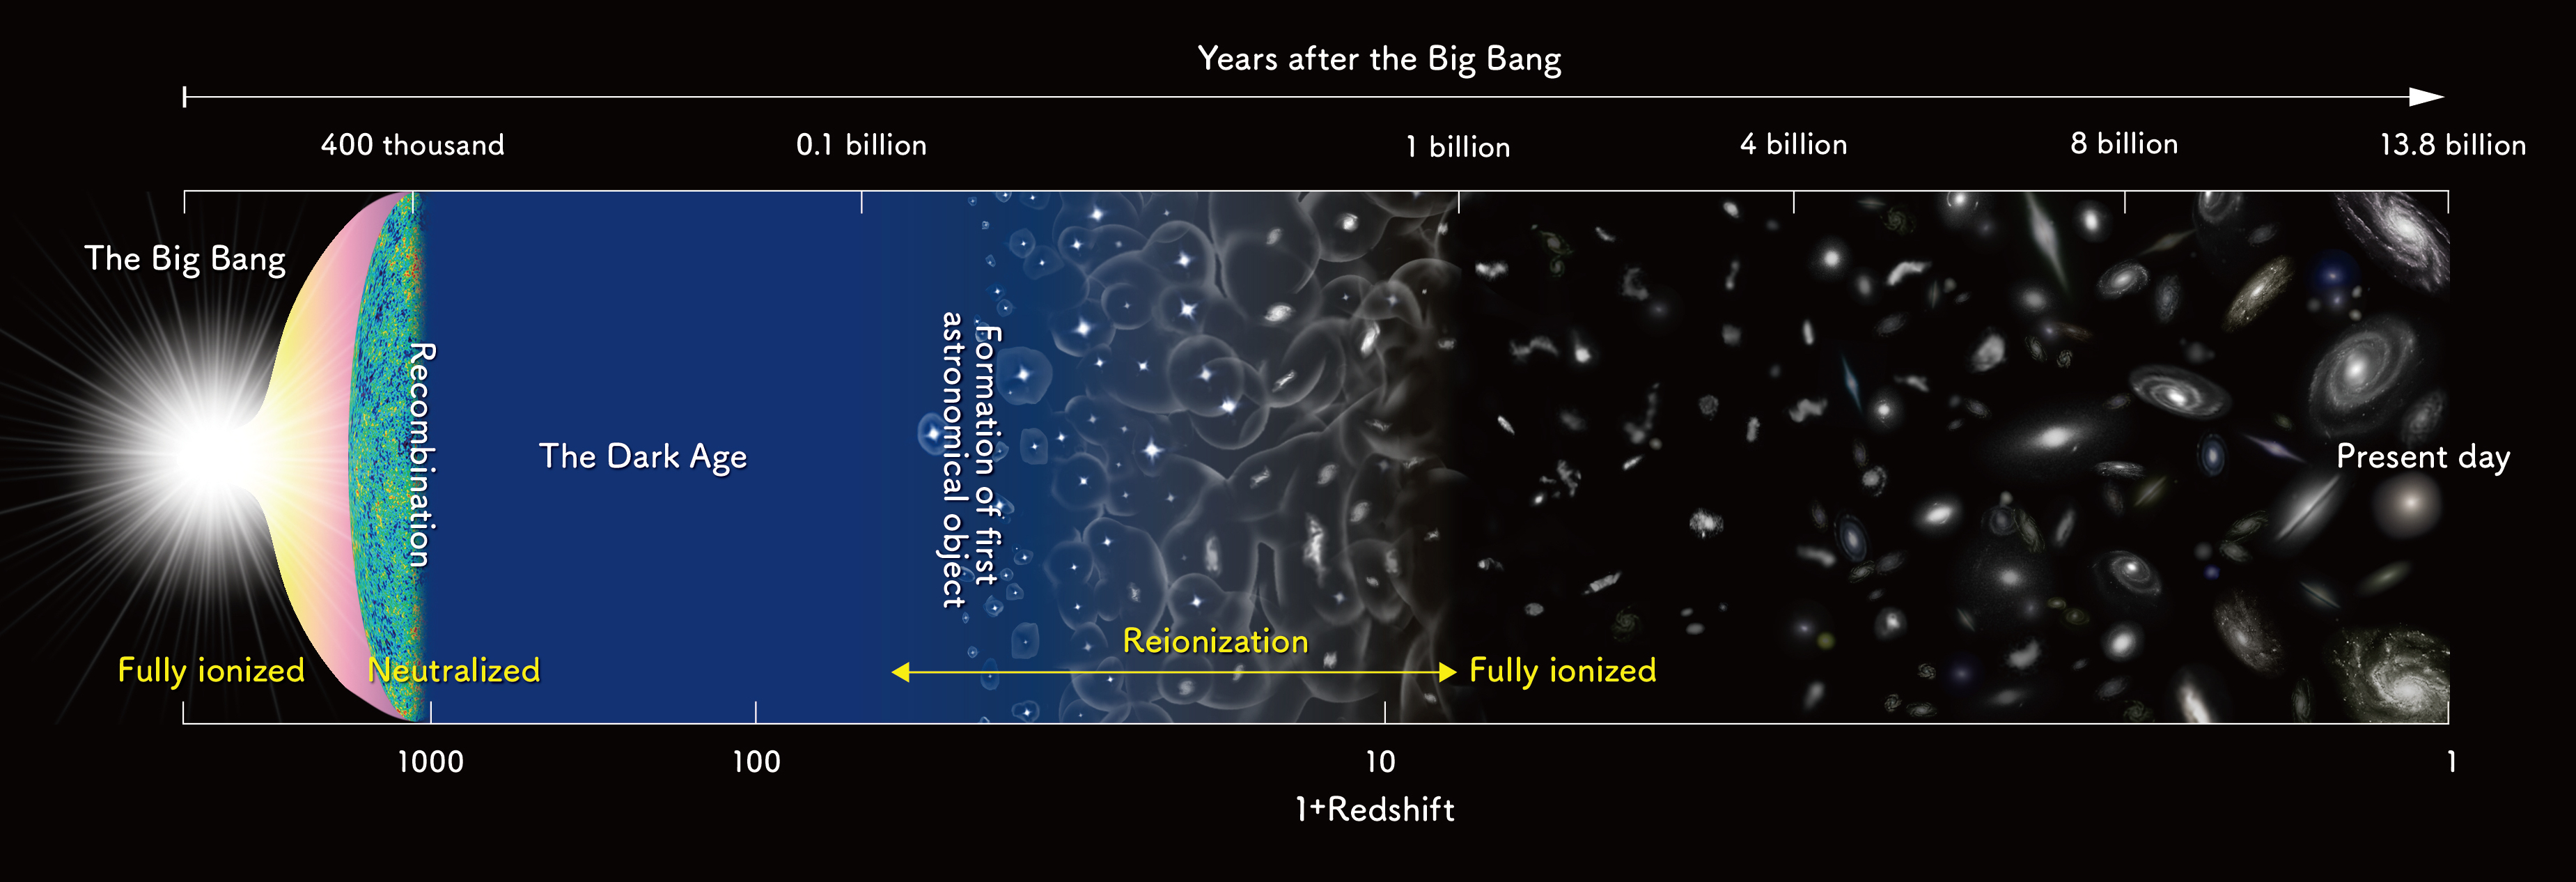
\includegraphics[width=1.0\textwidth]{intro/reionization.png}
	\caption[Epoch of Reionization Timeline]{Timeline of the history of the universe from its formation (left) to present day (right).}
	\label{fig:timeline}
\end{figure}



\begin{figure}[th]
	\centering
	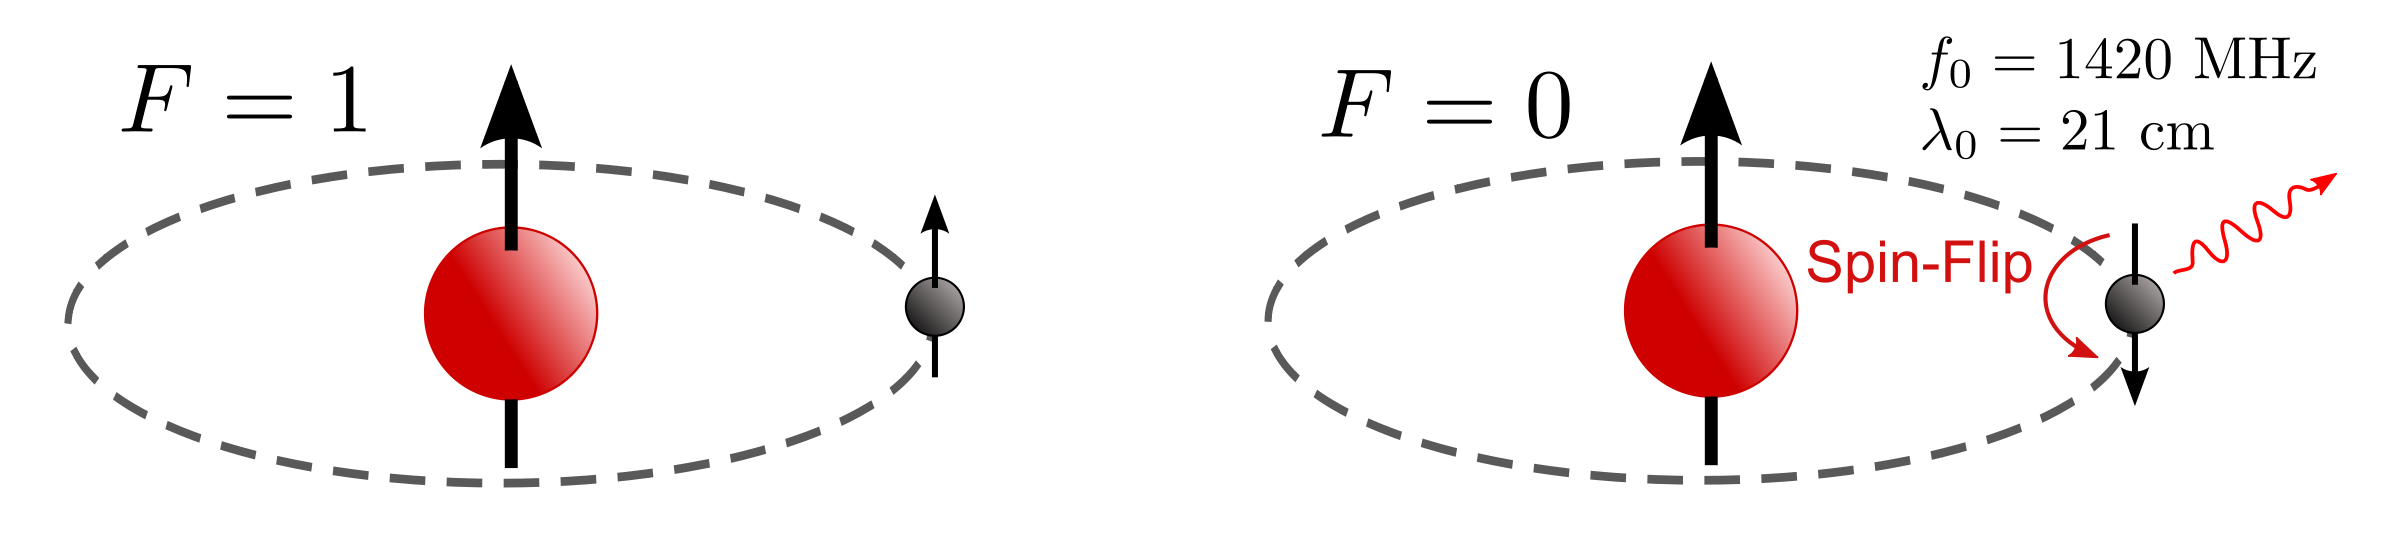
\includegraphics[width=0.90\textwidth]{spin_flip_H.png}
	\caption[Spin-Flip Transition of Neutral Hydrogen]{A depiction of the spin-flip transition of neutral hydrogen. Initially,
																					 the spin of the proton and electron are parallel and oriented
																					 in the same direction. The transition occurs when the electron's spin spontaneously
																					 flips from the higher energy parallel alignment to the lower energy anti-parallel alignment,
																					 releasing a photon with a wavelength of 21\,cm.}
	\label{fig:spin_flip}
\end{figure}

\begin{figure}[th]
	\centering
	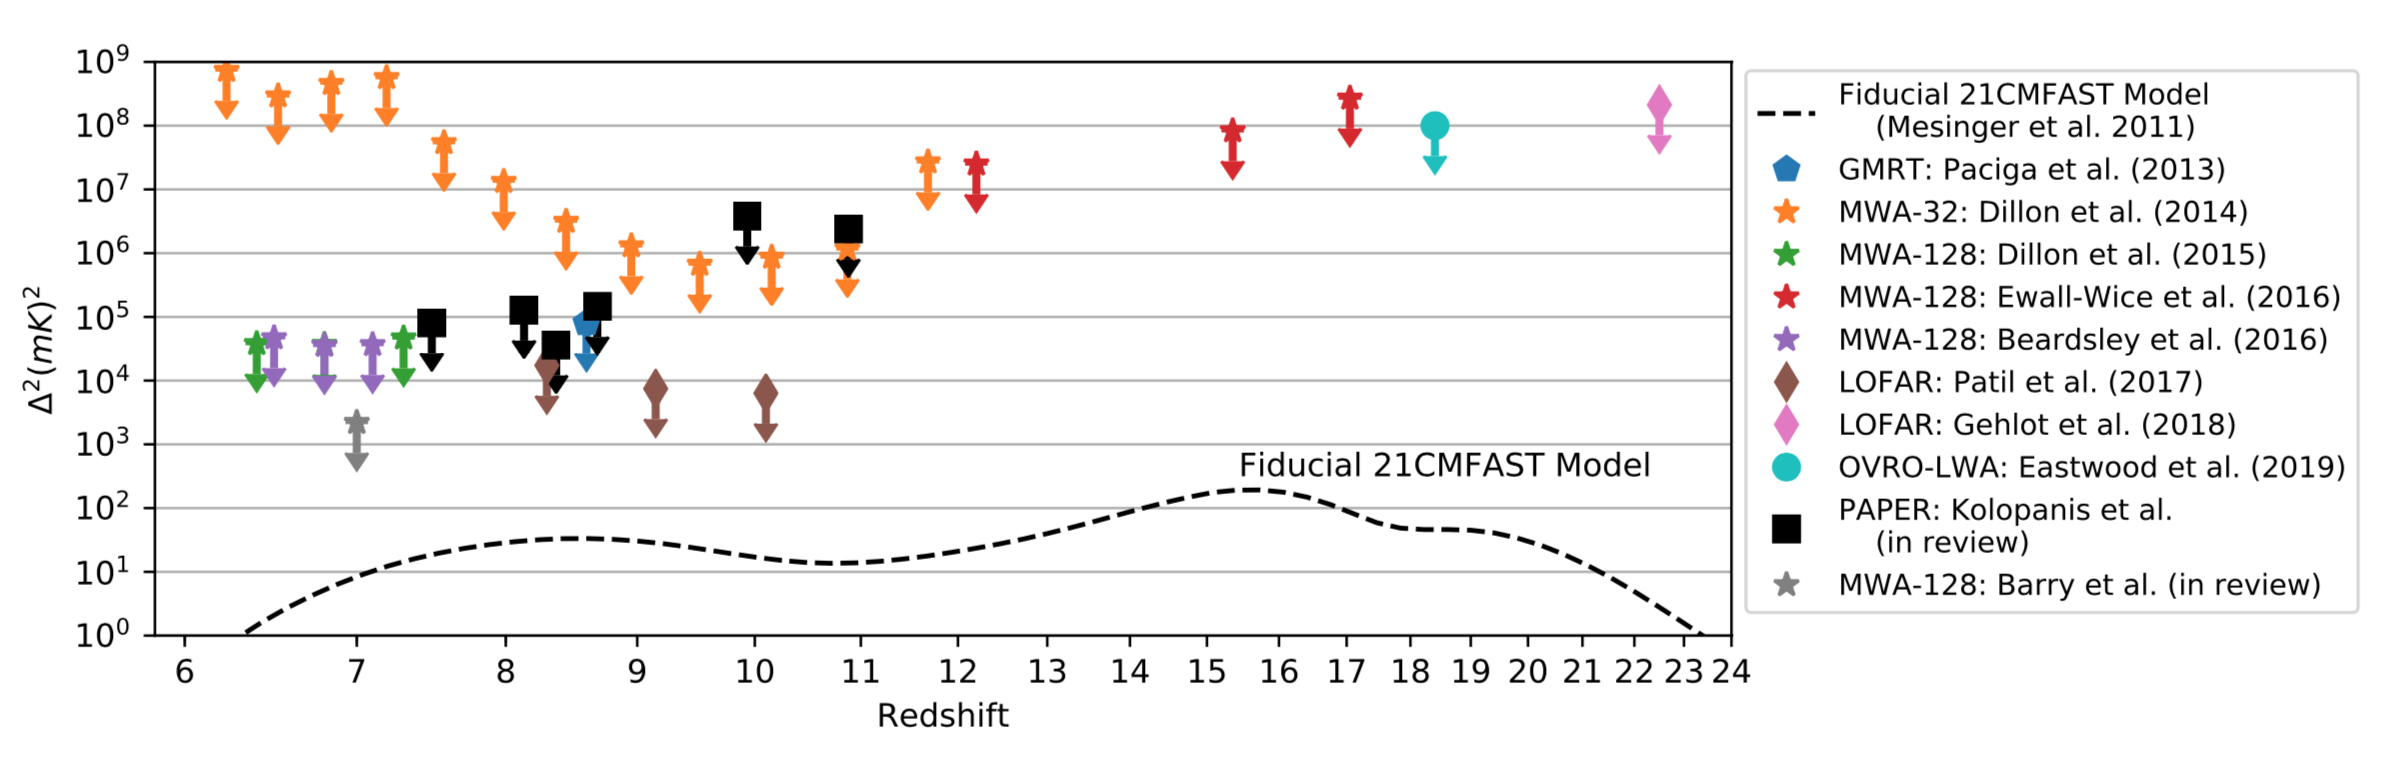
\includegraphics[width=1.\textwidth]{upper_limit.png}
	\caption[Upper Limits on Reionization]{A summary of the upper limits on the 21\,cm power spectrum across reionization. Plotted in the dashed line is a fiducial model of the 21\,cm power spectrum as simulated by \fastsim. Image taken from \cite{2019arXiv190708211L}}
	\label{fig:upper_limit}
\end{figure}


	\tocless\subsection{\hypertarget{subsec:eor}{1.3.\hspace{0.75em}}21cm Cosmology}
	\addcontentsline{toc}{subsection}{1.3.\hspace{0.75em}21cm Cosmology}

			\begin{figure}[th]
	\centering
	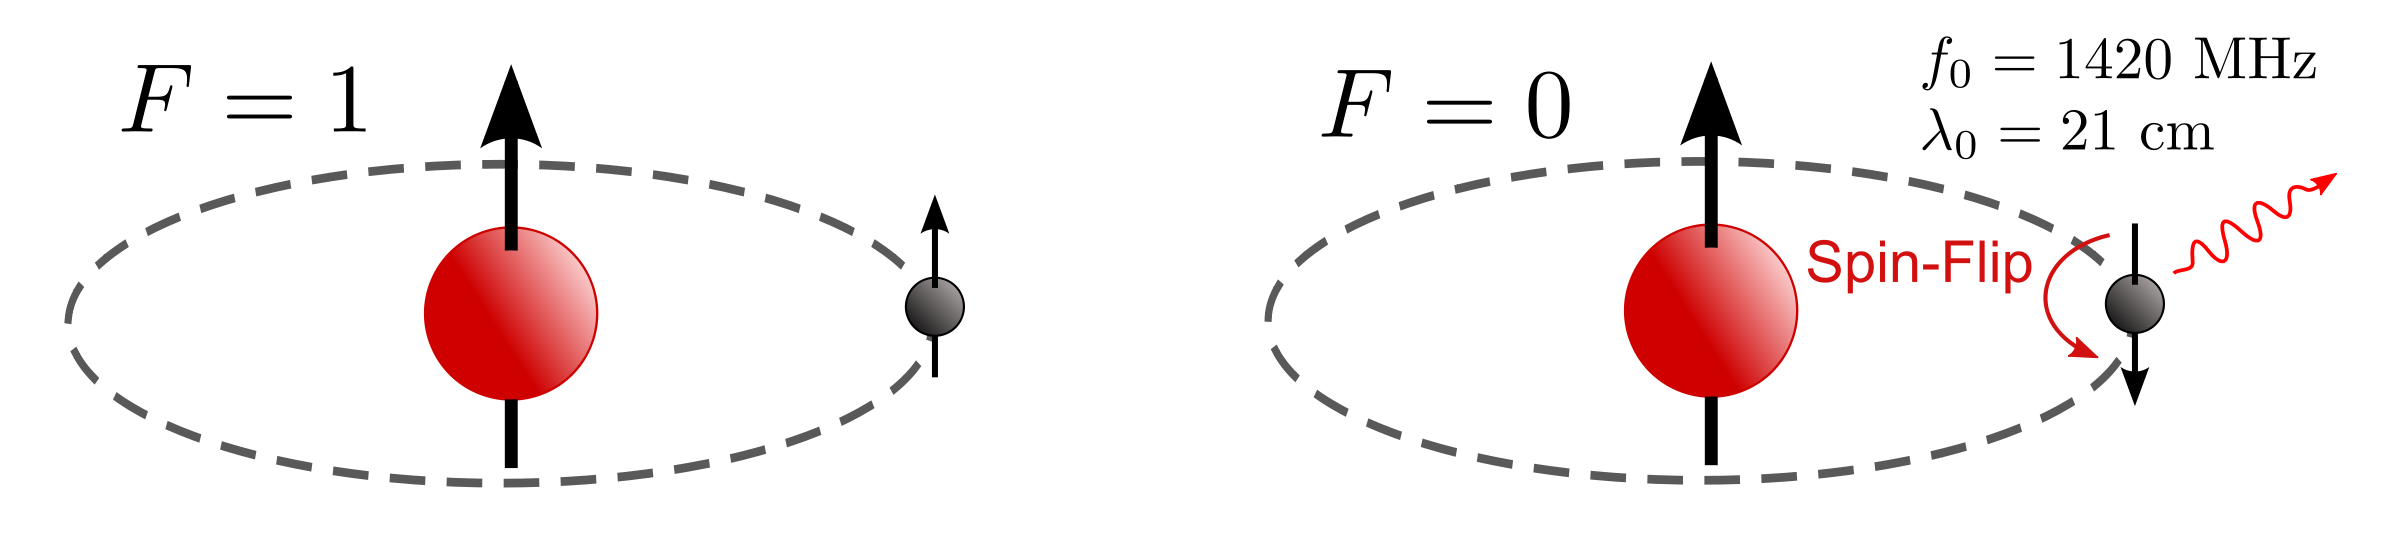
\includegraphics[width=0.95\textwidth]{spin_flip_H.png}
	\caption[Epoch of Reionization Timeline]{Depiction of the spin flip energy transition of neutral hydrogen}
	\label{fig:reionization}
\end{figure}



	\tocless\subsection{\hypertarget{subsec:hera}{1.4.\hspace{0.75em}The Hydrogen Epoch of Reionization Array}}
	\addcontentsline{toc}{subsection}{1.4.\hspace{0.75em}The Hydrogen Epoch of Reionization Array}

		\begin{figure}[th]
	\centering
	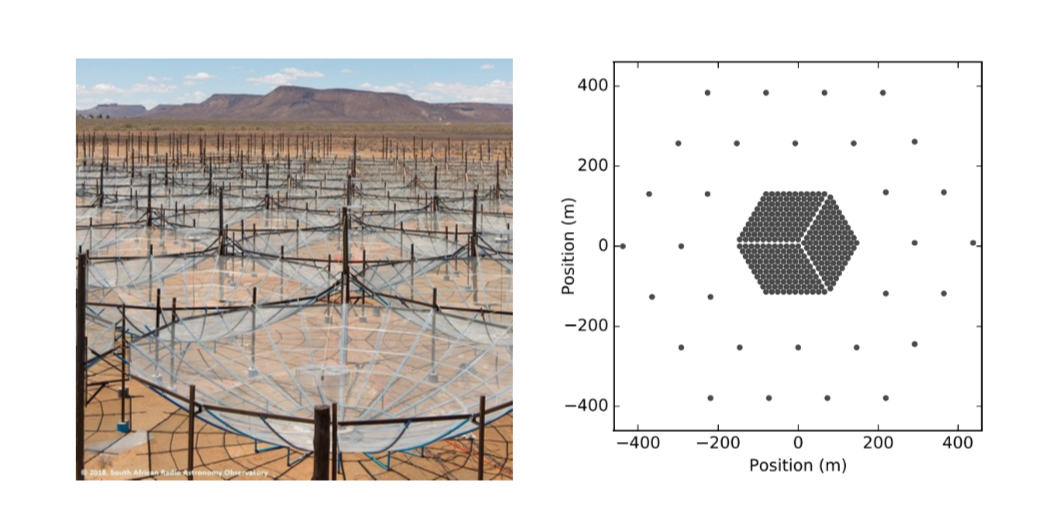
\includegraphics[width=0.95\textwidth]{intro/hera_layout.png}
	\caption[HERA Layout]{The power spectrum estimated after flagging a contiguous block of two channels.}
	\label{fig:hera_layout}
\end{figure}


\begin{figure}[th]
	\centering
	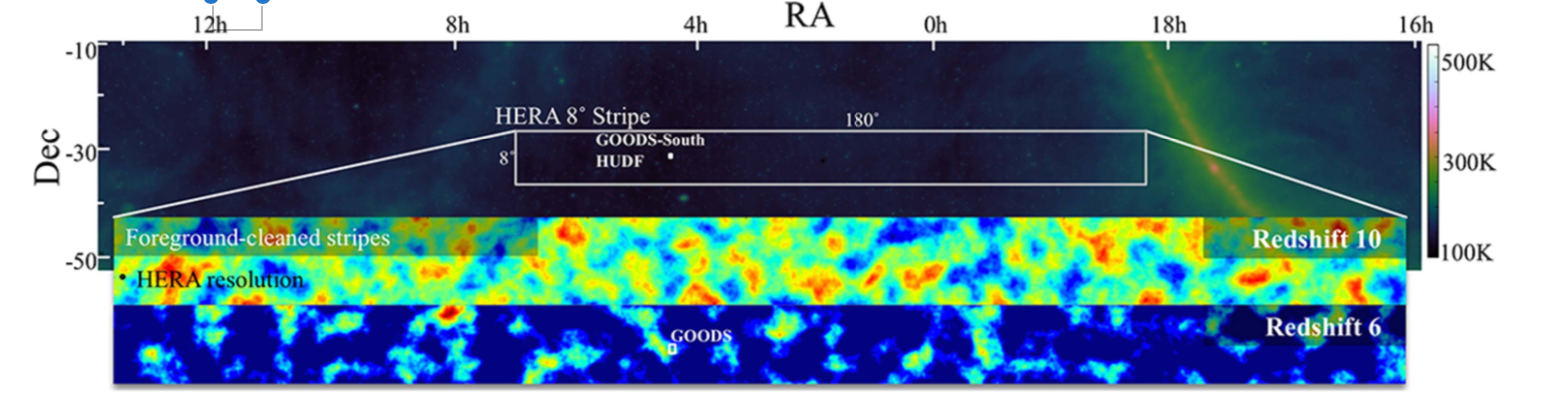
\includegraphics[width=0.95\textwidth]{intro/hera_stripe.png}
	\caption[HERA Field of View]{The power spectrum estimated after flagging a contiguous block of two channels.}
	\label{fig:hera_stripe}
\end{figure}



	\tocless\subsection{\hypertarget{subsec:spherex}{1.4.\hspace{0.75em}SPHEREx}}
	\addcontentsline{toc}{subsection}{1.2.\hspace{0.75em}SPHEREx}

		In addition using the 21\,cm line to characterize the EoR, intensity mapping of the
\lya\ transition of neutral hydrogen will provide a wealth of information about
the state of reionization. The \lya\ line has been shown to be a tracer of high-redshift
galaxies and the bubble of ionized gas around them in \cite{2013ApJ...763..132S} and \cite{2014ApJ...786..111P}.
A number of experiments look to probe reionization through the \lya\ line, but the most
prominent experiment of its kind planned for launch is that of the Spectro-Photometer
for the History of the Universe, Epoch of Reionization, and Ices Explorer (SPHEREx),
\cite{2014arXiv1412.4872D}.

\begin{figure}[th]
	\centering
	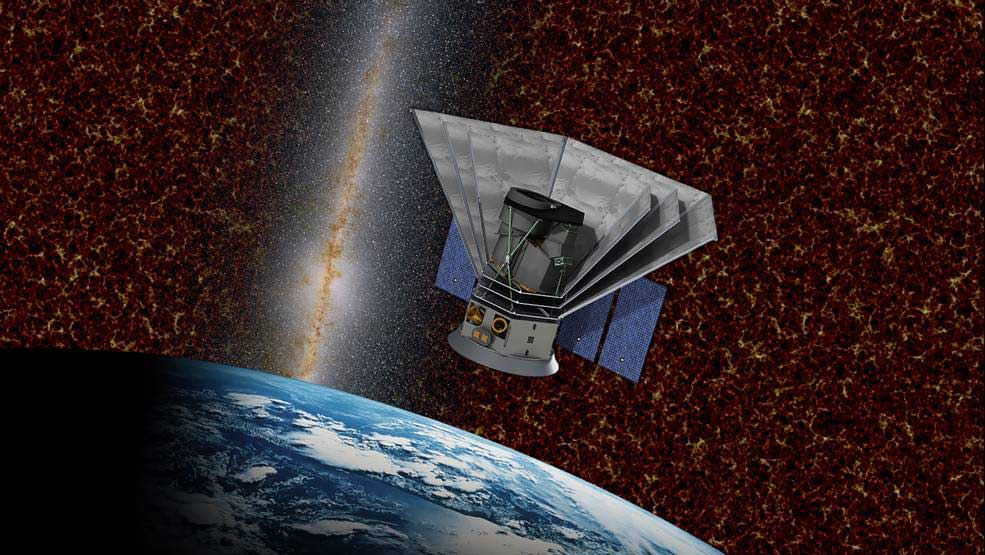
\includegraphics[width=0.95\textwidth]{spherex.jpg}
	\caption[SPHEREx Instrument]{Simulated image of the SPHEREx probe in orbit.}
	\label{fig:spherex}
\end{figure}

SPHEREx is a near-infrared, space-based observatory whose primary science goal is to perform
an all-sky survey in near-infrared bands of 450 million galaxies to constrain the
physics of inflation using the large-scale structure of these galaxies. While not
the primary goal of the mission, SPHEREx also looks to do intensity mapping of the
\lya\ line to study the origin and evolution of early galaxies. With a target launch
date set for December 2023, SPHEREx may provide the very first \lya\ intensity mapping
measurements during reionization. Given its sensitivity and frequency range, SPHEREx should
be able to detect these EoR fluctuations over the redshift range $z \approx 6 - 8$.









%----------------------------------%
%							Methods							 %
%----------------------------------%

\tocless\section{\hypertarget{sec:methods}{2.\hspace{0.75em}Methods}}
\addcontentsline{toc}{section}{2.\hspace{0.75em}Methods}

\tocless\subsection{\hypertarget{subsec:methods}{2.1.\hspace{0.75em}21cmFAST}}
\addcontentsline{toc}{subsection}{2.1.\hspace{0.75em}21cmFAST}

	\label{sec:21cm_temp}

In this subsection, I briefly describe the simulation of the 21\,cm cosmological
signal. As mentioned in the previously, \fastsim\ was written specifically to simulate the 21\,cm
signal. It does this by generating density, velocity, and ionization fields at $z \approx 35$ and evolving
them through cosmic time. With these fields and the following expression, the brightness temperature offset of the
21\,cm signal can then be evaluated at a given redshift.
\begin{align}
  \delta T_b \left(z \right) & = \frac{T_S - T_{\gamma}}{1+z} \left(1 - e^{-\tau_{\nu_0}} \right ) \nonumber \\
      & \approx 27 x_{\rm HI} \left( 1 + \delta_{\rm nl} \right) \left( \frac{H}{dv_r/dv + H}\right) \left( 1 - \frac{T_{\gamma}}{T_S}\right) \nonumber \\
      & \hspace{1em} \times \left( \frac{1 + z}{10} \frac{0.15}{\Omega_{\rm M} h^2} \right)^{1/2} \left( \frac{\Omega_{\rm b} h^2}{0.023} \right) \textrm{ mK,}
      \label{eqn:offset_temp}
\end{align}
In the equation above, $T_S$ is the gas spin temperature, $T_{\gamma}$ is the
CMB temperature, $\tau_{\nu_0}$ is the optical depth at 21cm frequency, $\delta_{\rm nl} = \rho / \bar{\rho}_0 - 1$
is the non-linear density contrast $H \left( z \right)$
is the Hubble parameter, $dv_r / dr$ is the comoving gradient of the line of sight component
of the comoving velocity, where all quantities are evaluated at redshift $z = \nu_0 / \nu - 1$.
The brightness temperature offset can then be converted to a fluctuation field
for cross-correlation using the equation below,
\begin{equation}
\delta_{21} \left( \mathbf{x}, z\right) = \frac{ \delta T_b \left( \mathbf{x}, z\right)}{\delta \overline{T}_b \left( z \right)} - 1,
\end{equation}
where $\delta \overline{T}$ is the spatial average of the 21\,cm brightness temperature offset
$\delta T \left( \mathbf{x}, z\right)$. The simulated 21\,cm brightness temperature offset field defined
in Equation \ref{eqn:offset_temp} can be see in Figure \ref{fig:sims}.


\tocless\subsection{\hypertarget{subsec:methods}{2.2.\hspace{0.75em}Power Spectrum}}
\addcontentsline{toc}{subsection}{2.2.\hspace{0.75em}Power Spectrum}

		\begin{equation}
\langle \widetilde{\delta}_i ({\bf k}) \widetilde{\delta}_j ({\bf k'}) \rangle = (2 \pi) ^3 \delta_D \left( {\bf k} - {\bf k'} \right) P_{ij} \left({\bf k} \right)
\end{equation}

\begin{equation}
    \widetilde{\Delta} \left( k \right) = \frac{k^3}{2 \pi ^2} P \left( k \right)
\end{equation}

\begin{equation}
    \Delta \left( k \right) = \left( \nu I_{\nu} \right)^2 \widetilde{\Delta} \left( k \right)
\end{equation}s

\begin{figure}[ht]
	\centering
	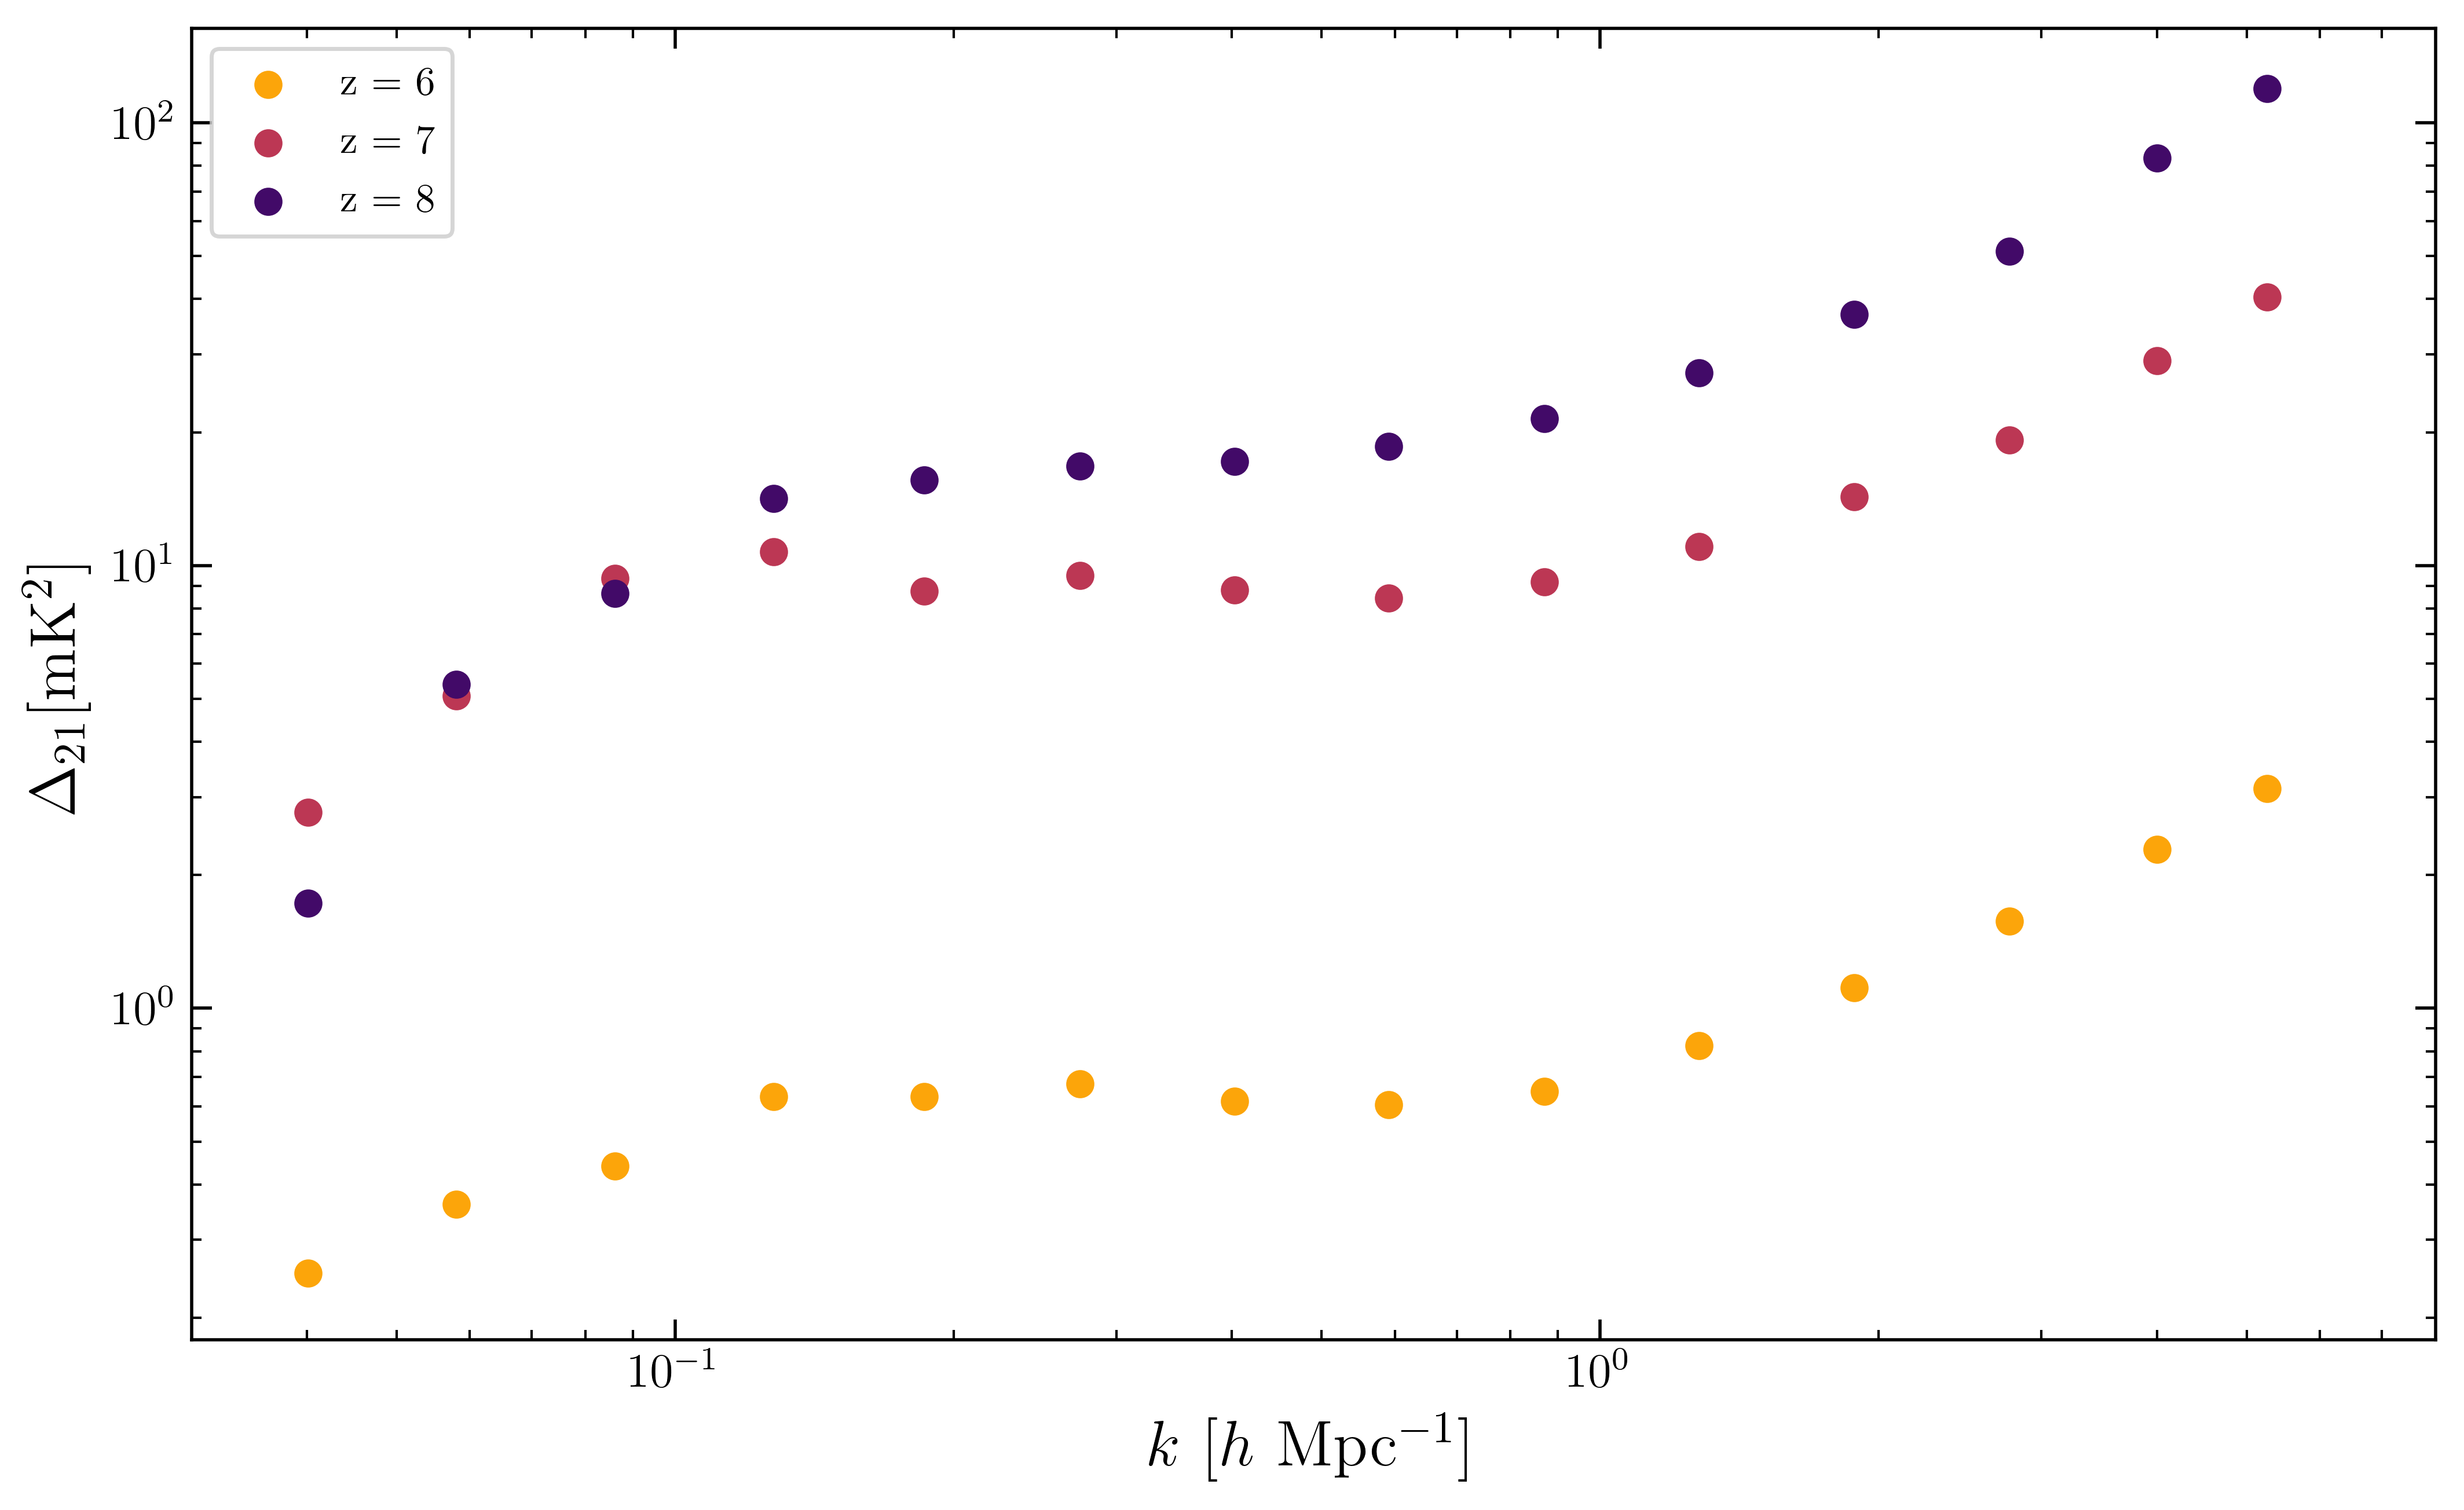
\includegraphics[width=0.9\textwidth]{21cm_power_spectrum.png}
	\caption[21cm Power Spectrum]{Cross-correlation coefficient}
	\label{fig:21cm_ps}
\end{figure}

\begin{figure}[ht]
	\centering
	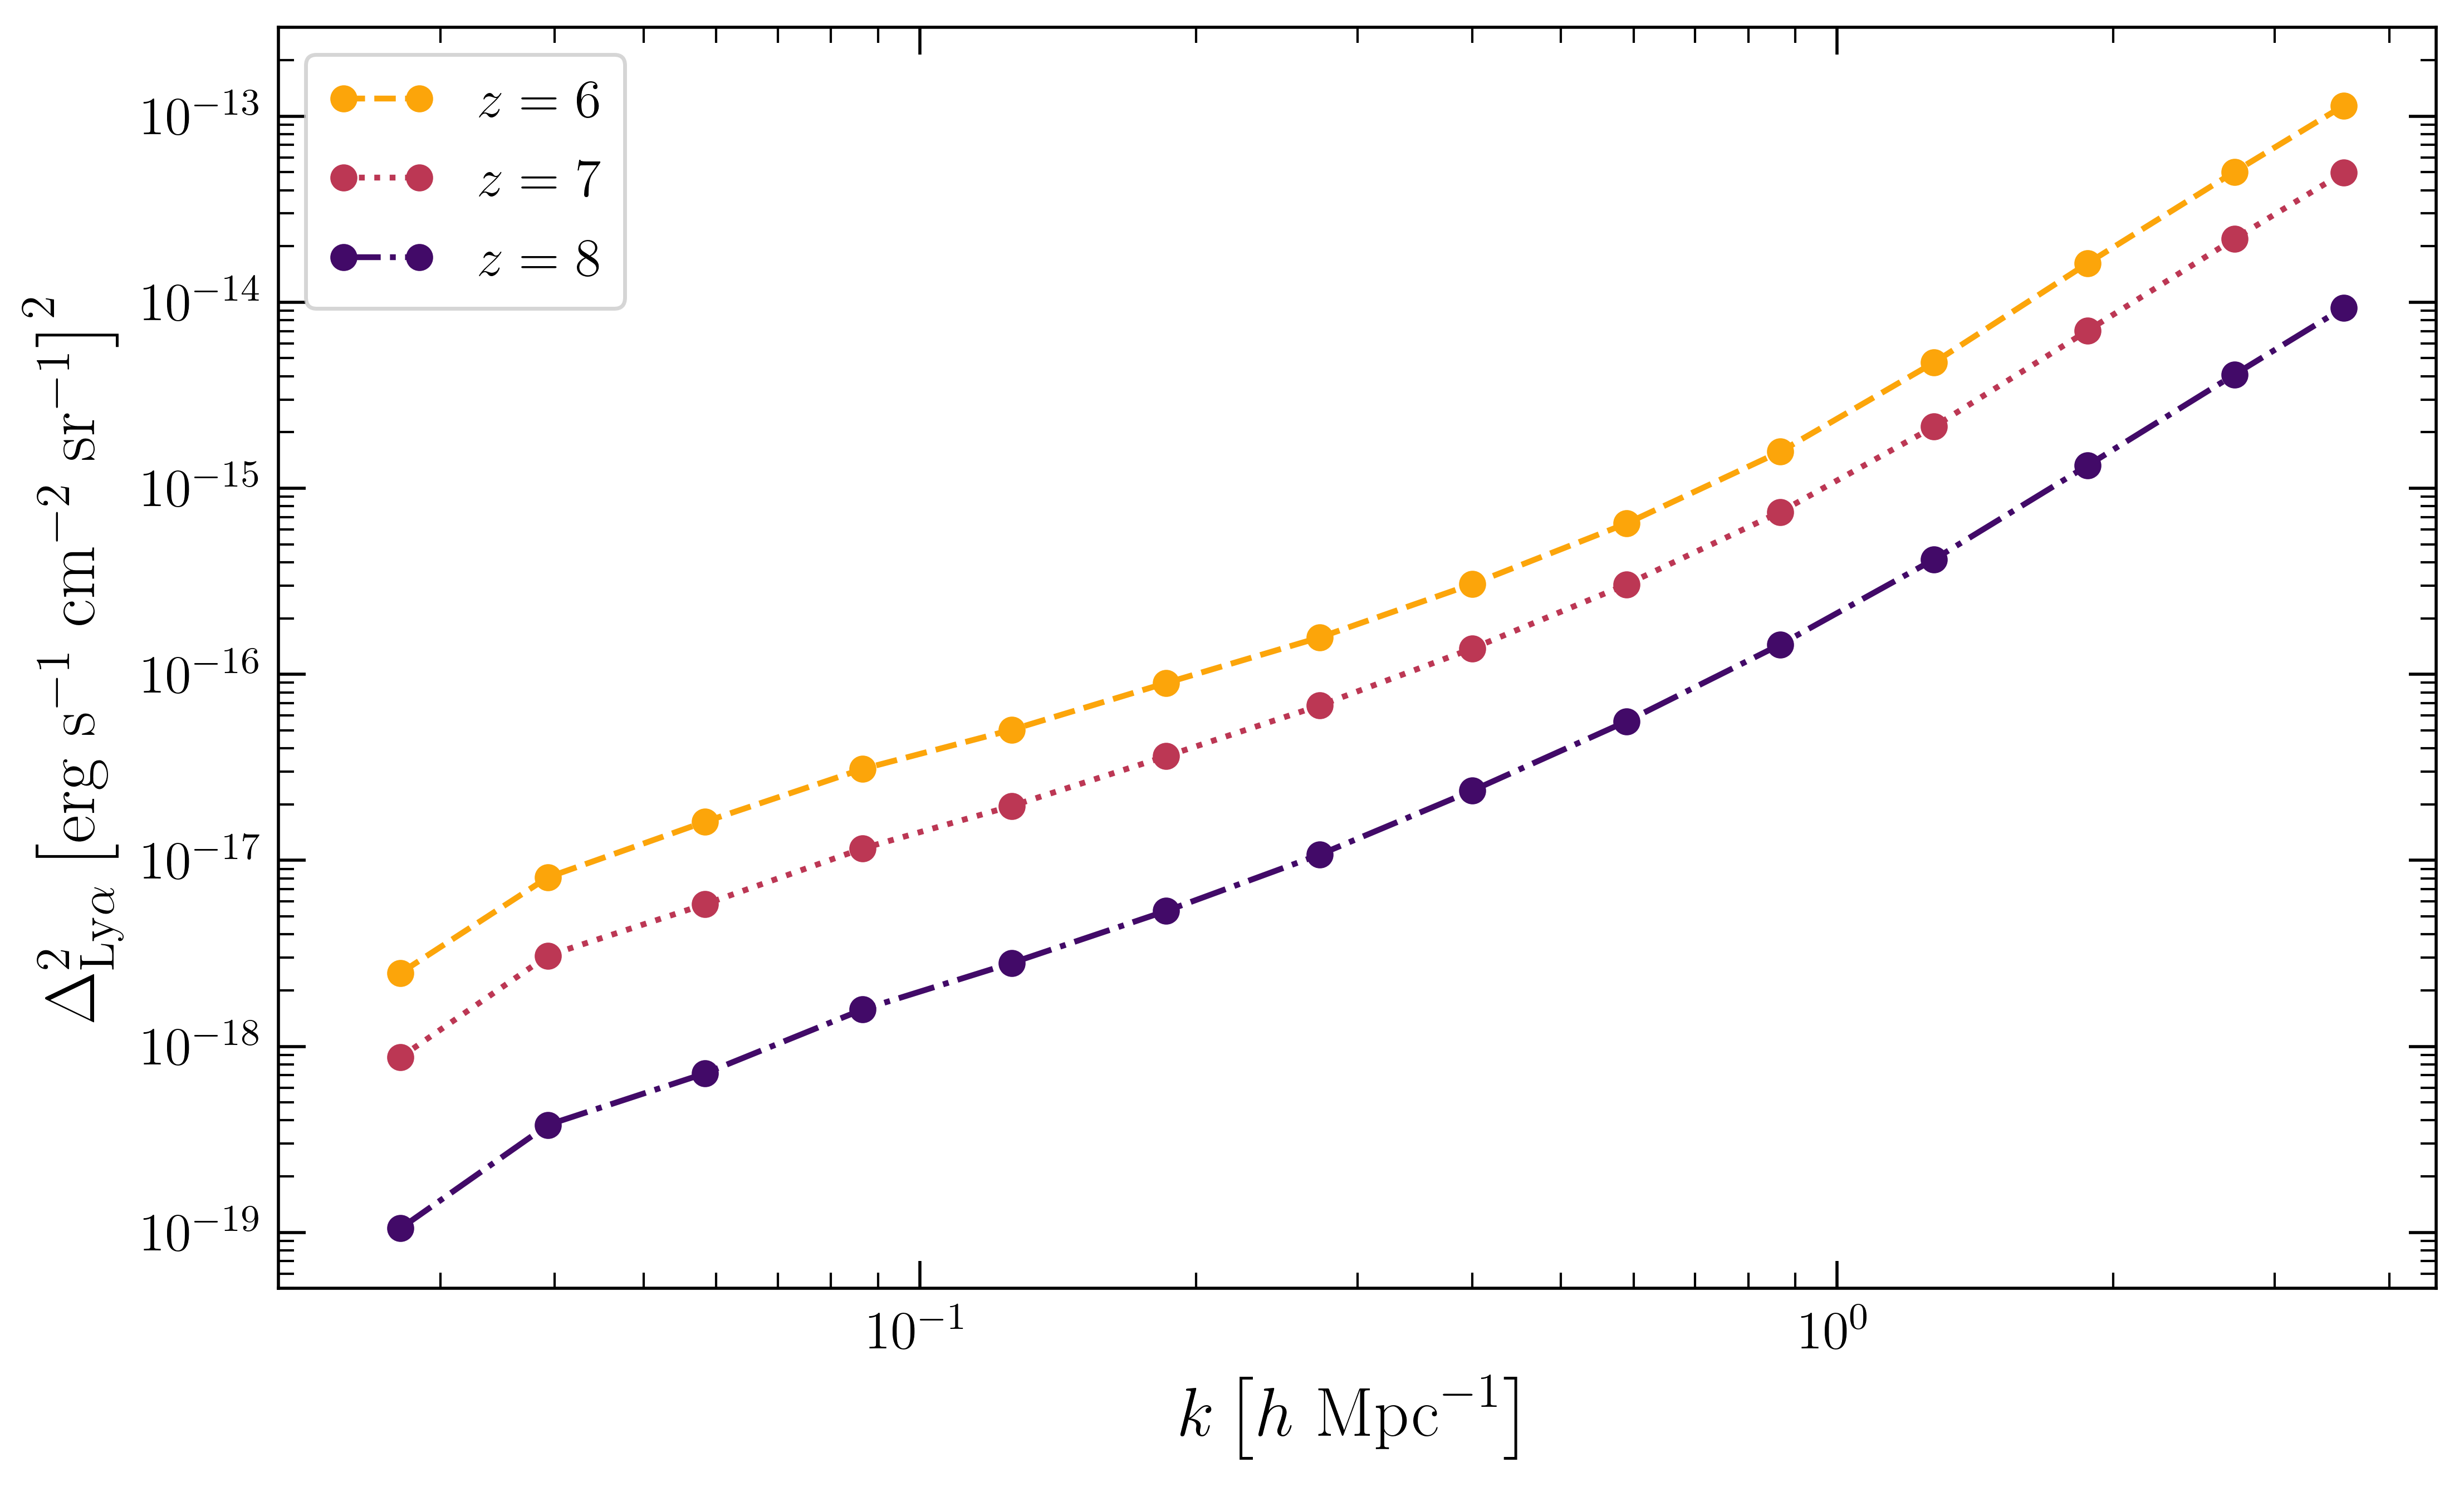
\includegraphics[width=0.9\textwidth]{lyman_alpha_pspec.png}
	\caption[Ly$\alpha$ Power Spectrum]{Cross-correlation coefficient}
	\label{fig:lya_ps}
\end{figure}

\begin{figure}[ht]
	\centering
	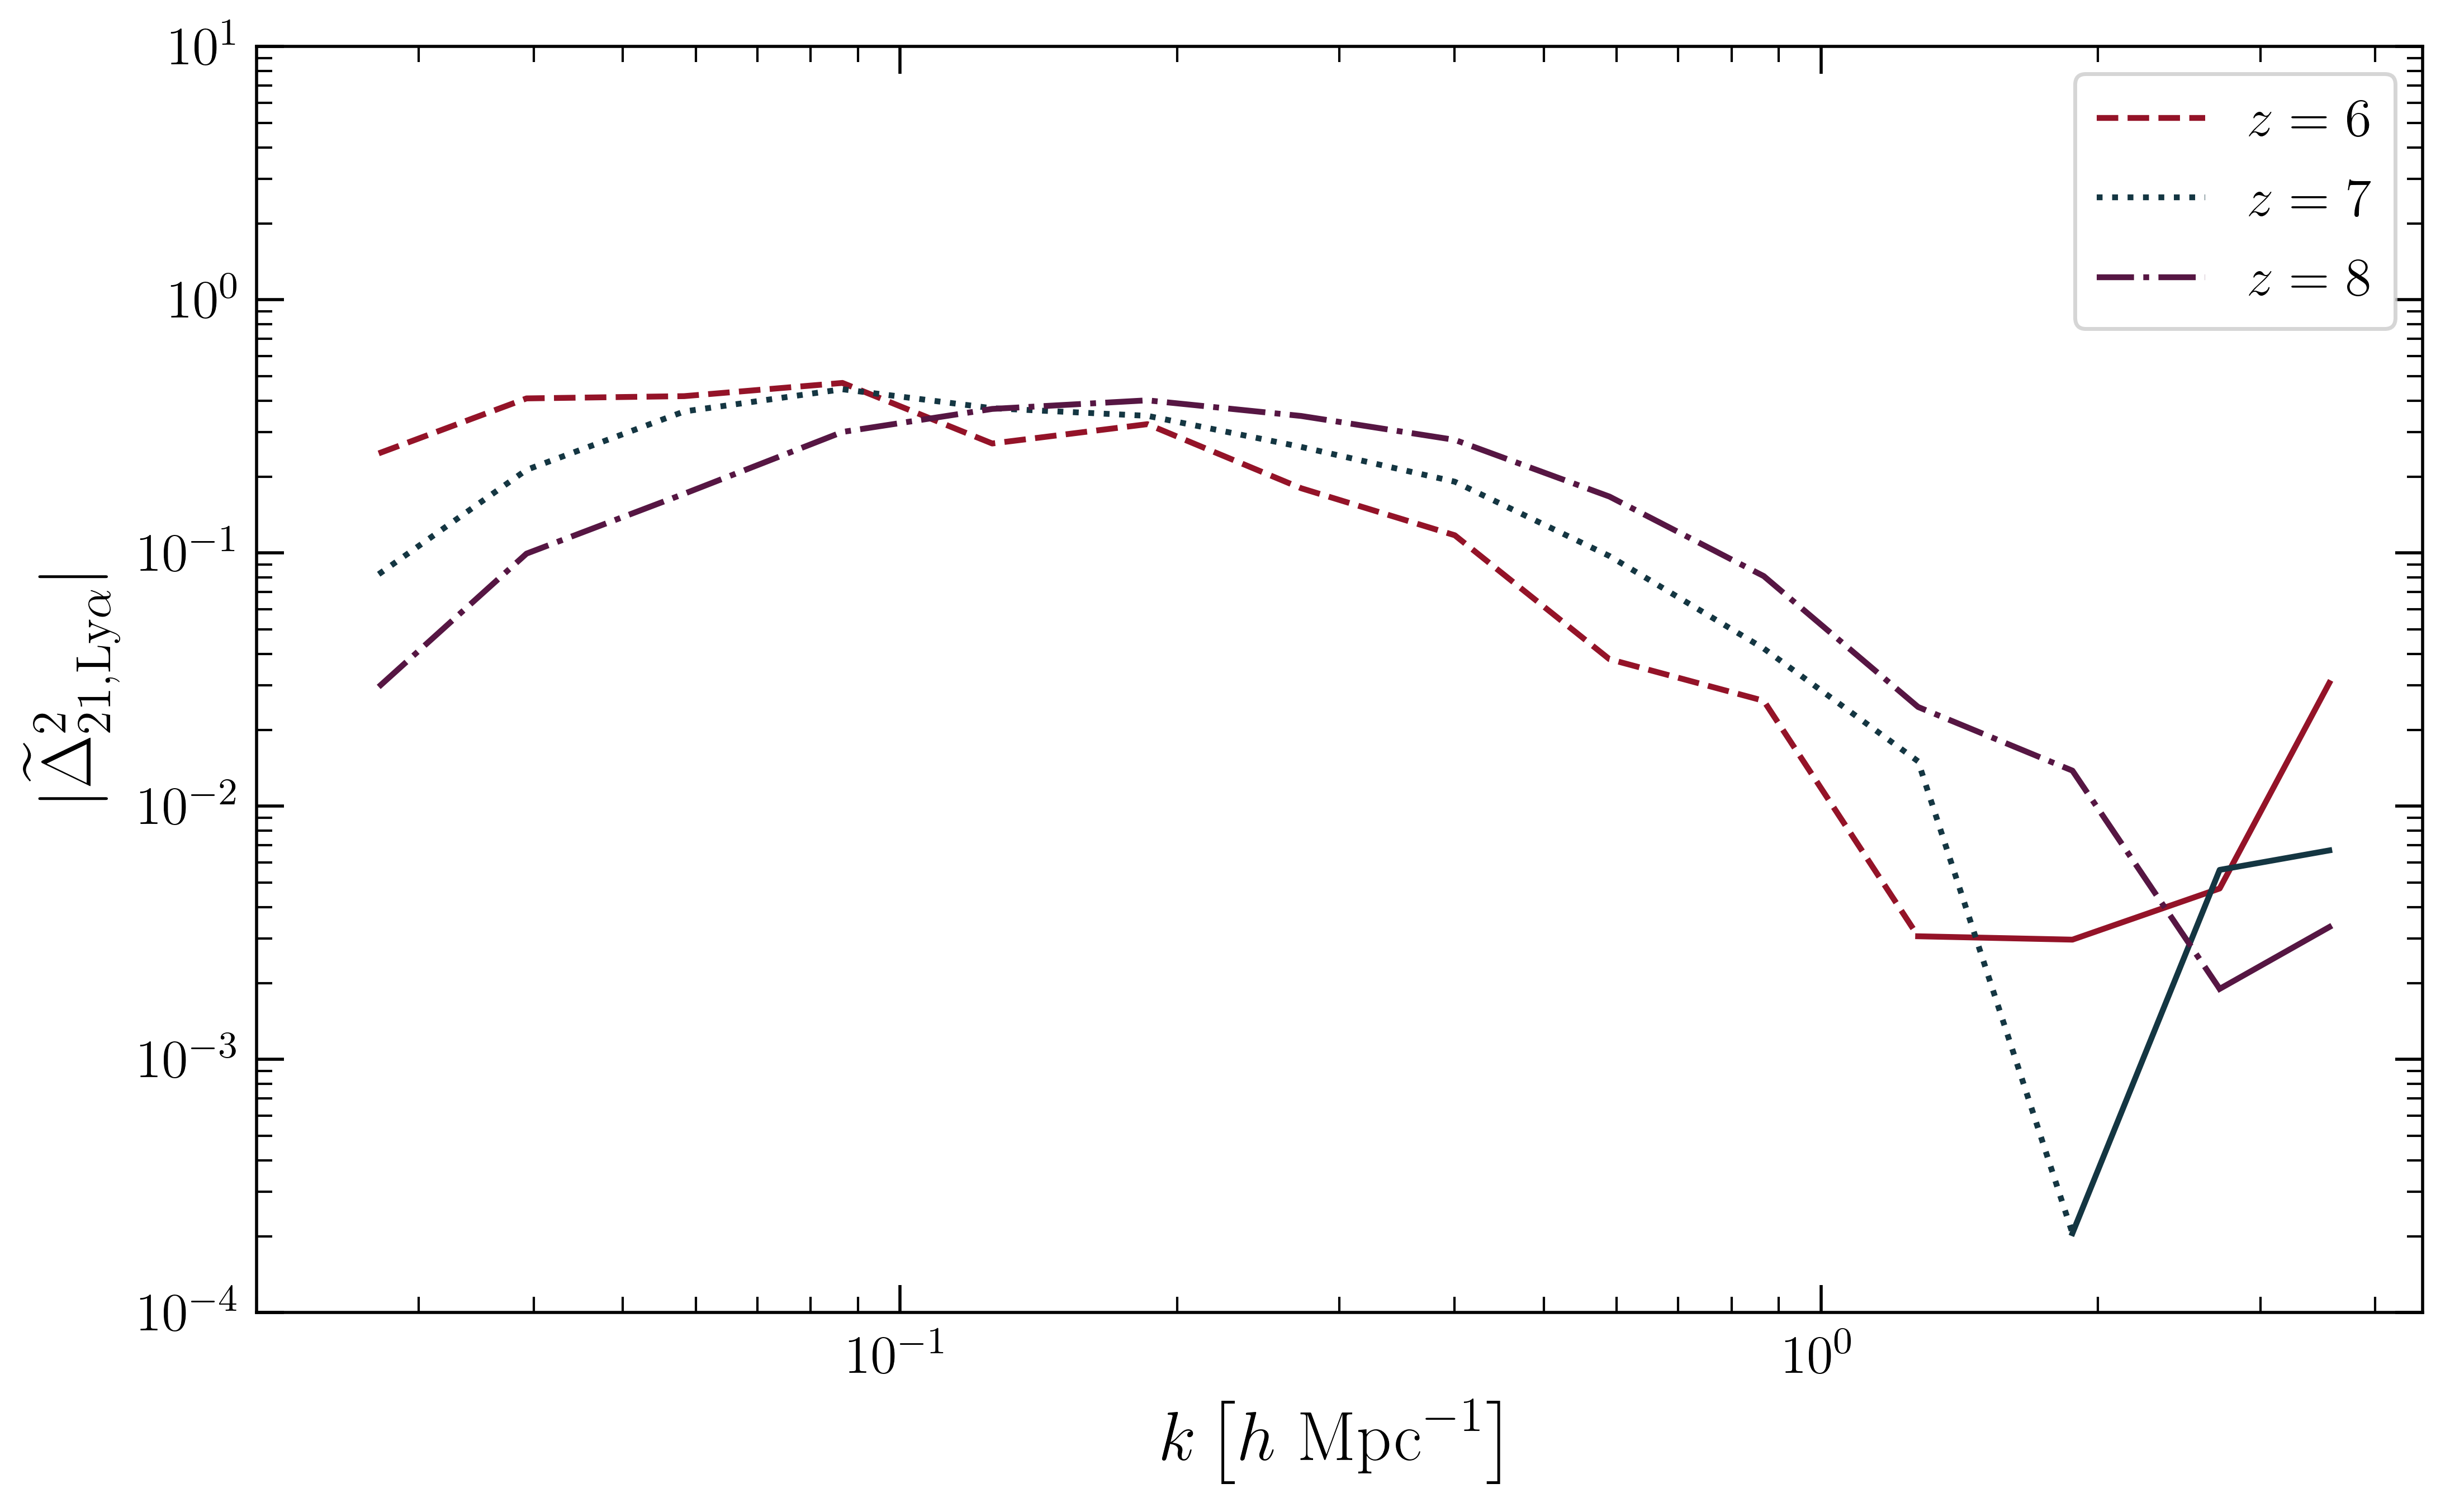
\includegraphics[width=0.9\textwidth]{cross_power_spec.png}
	\caption[Cross-Power Spectrum]{Cross-correlation coefficient}
	\label{fig:x_ps}
\end{figure}

\begin{figure}[ht]
	\centering
	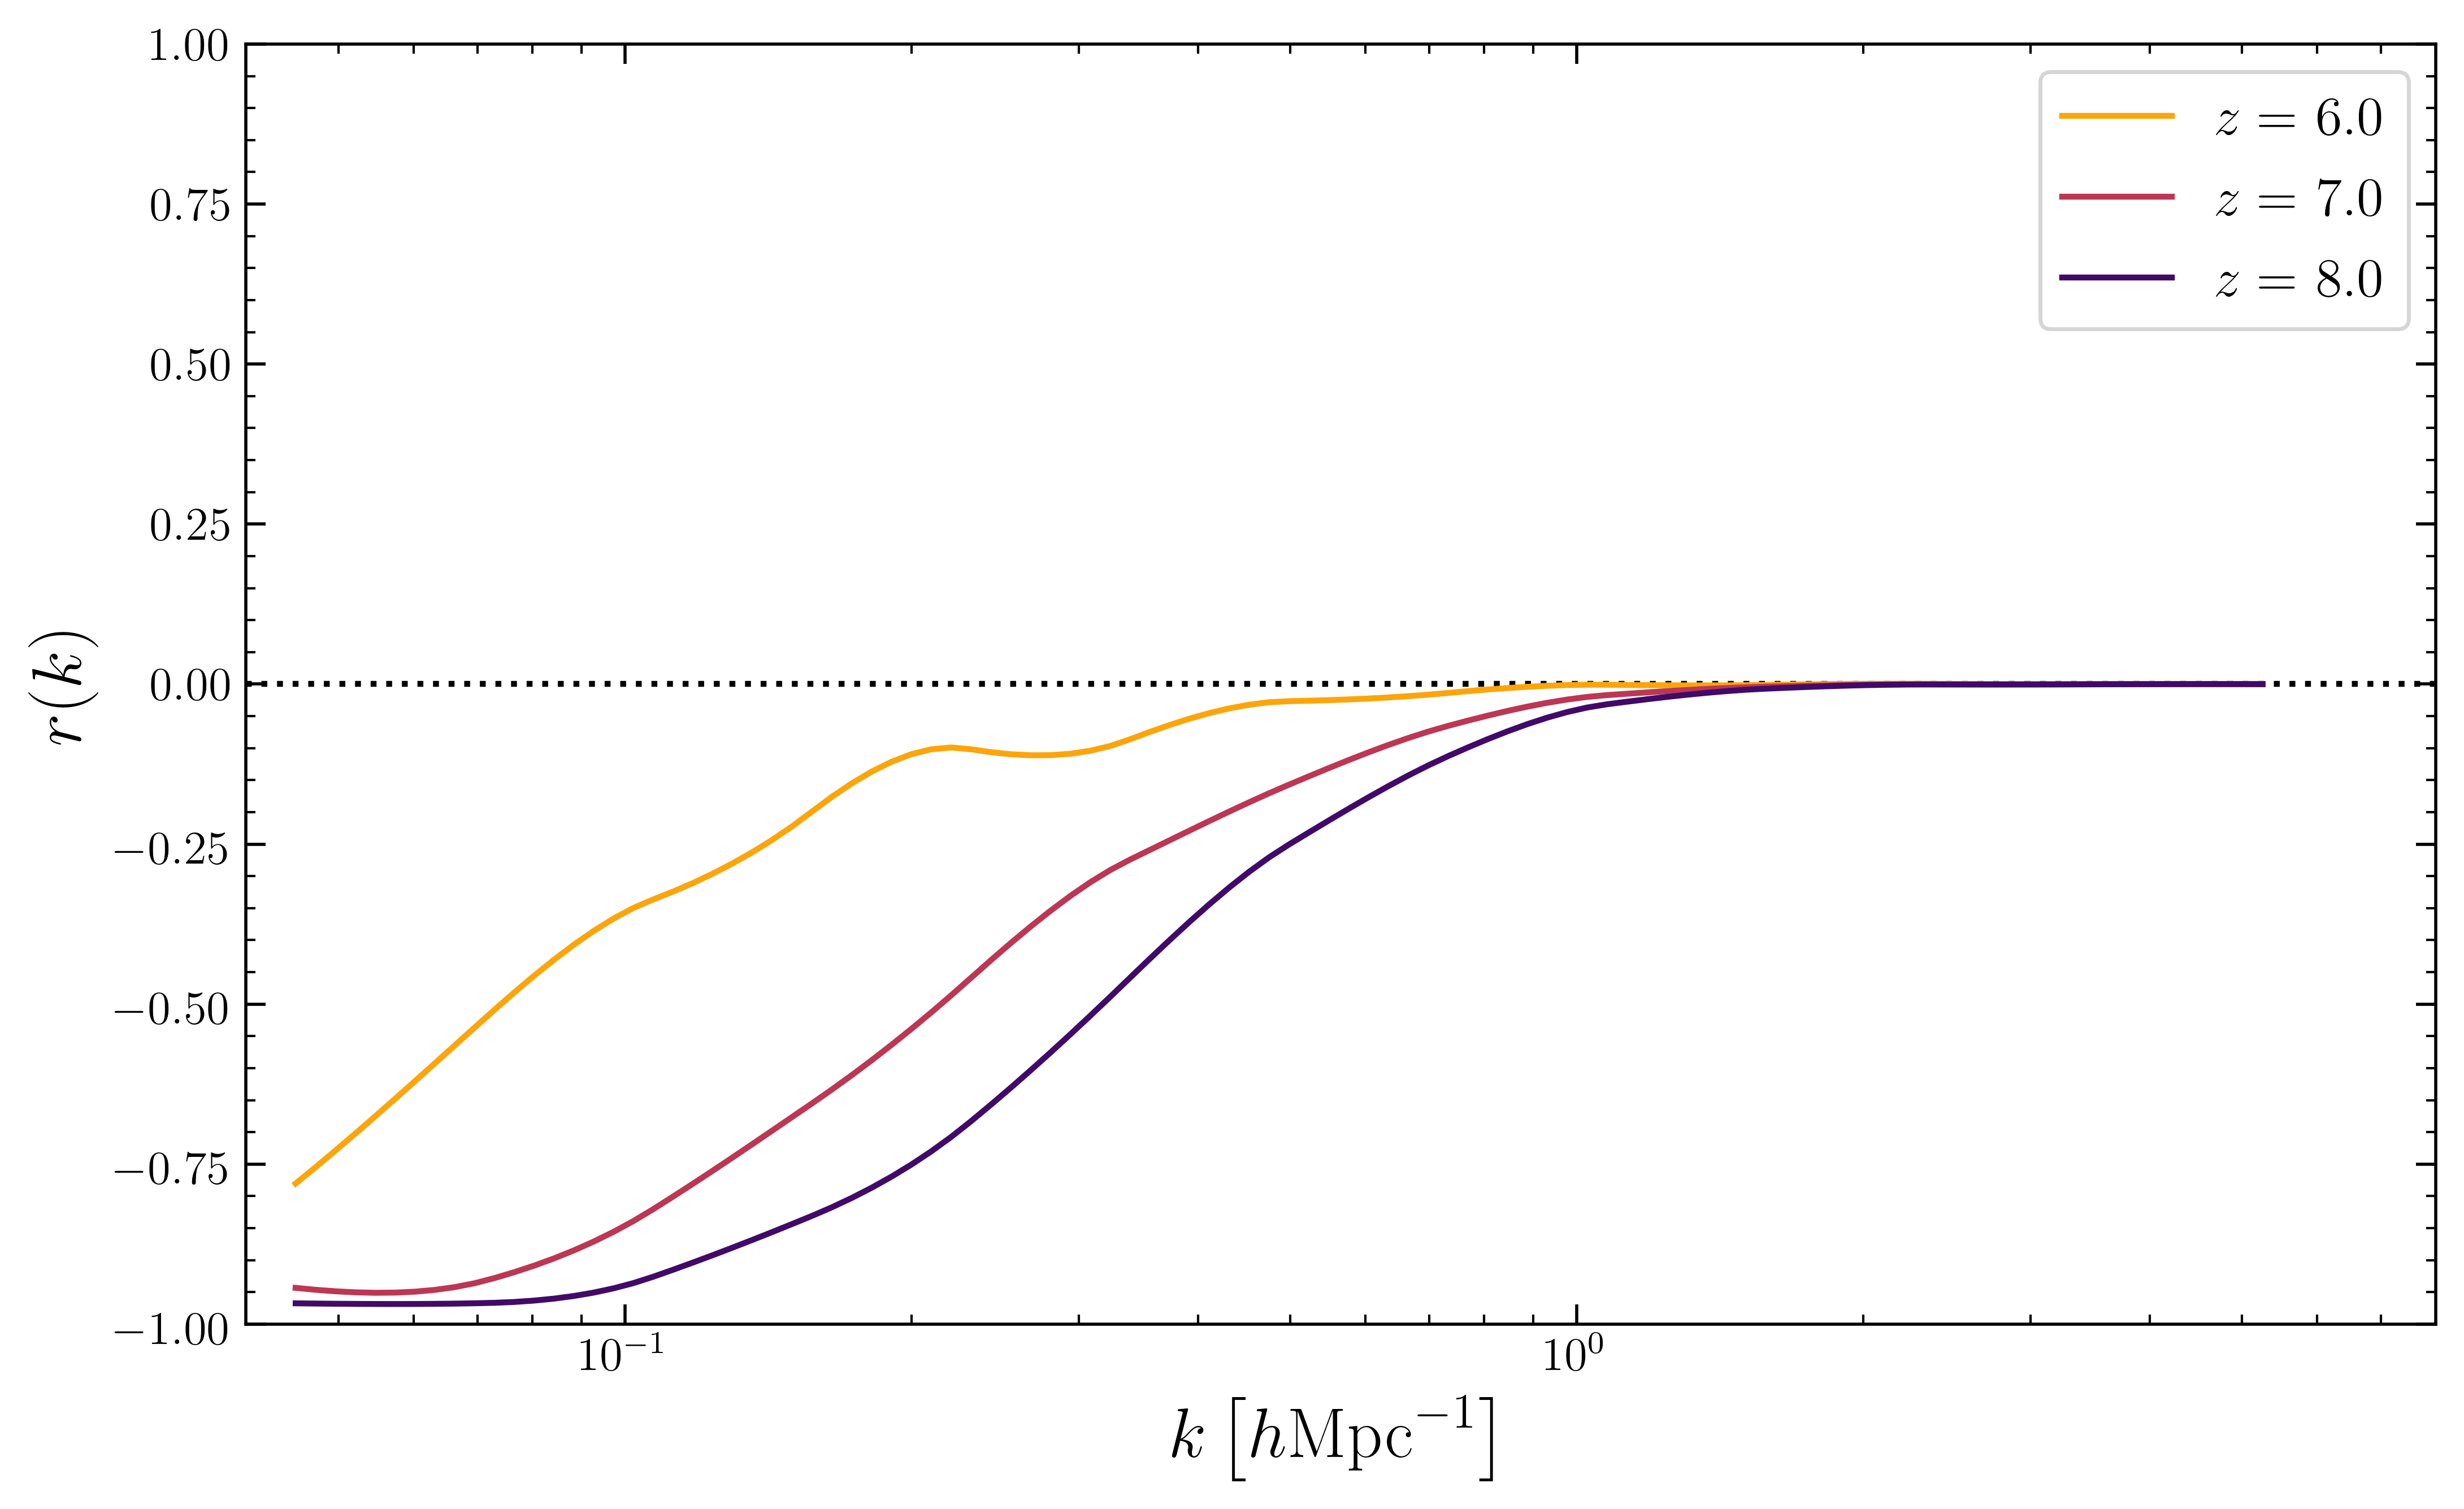
\includegraphics[width=0.9\textwidth]{ccc_plot.png}
	\caption[Cross-Correlation Coefficient]{Cross-correlation coefficient}
	\label{fig:ccc}
\end{figure}


\tocless\subsection{\hypertarget{subsec:methods}{2.2.\hspace{0.75em}21cm Noise Auto Spectrum}}
\addcontentsline{toc}{subsection}{2.2.\hspace{0.75em}21cm Noise Auto Spectrum}

	\begin{equation}
    2 \sigma^2_{21, \rm Ly\alpha} = P^2_{21, \rm Ly\alpha} +
      \left(P_{21} + \sigma_{21} \right) \left( P_{\rm Ly\alpha} + \sigma_{\rm Ly\alpha}\right)
\end{equation}


\tocless\subsection{\hypertarget{subsec:methods}{2.3.\hspace{0.75em}Ly$\alpha$ Noise Auto Spectrum}}
\addcontentsline{toc}{subsection}{2.3.\hspace{0.75em}Ly$\alpha$ Noise Auto Spectrum}

	\begin{equation}
P_{N, Ly\alpha} = \sigma_{\rm N}^2 V_{\rm vox}
\end{equation}

$V_{\rm vox} = A_{\rm pix} r_{\rm pix}$

\begin{equation}
\sigma_{Ly\alpha}^2 = \left[ P_{Ly\alpha}\left(k, \mu \right) + \sigma_{\rm N}^2 V_{\rm vox} {\rm W}_{Ly\alpha}\left(k, \mu \right) \right]
\end{equation}








%----------------------------------%
%							Results							 %
%----------------------------------%

\tocless\section{\hypertarget{sec:results}{3.\hspace{0.75em}Results}}
\addcontentsline{toc}{section}{3.\hspace{0.75em}Results}

\begin{table}[]
\begin{tabularx}{\textwidth}{ccccccc}
\hline
\hline
\centering
\begin{tabular}[c]{@{}c@{}}$\nu_{res}$ \\ (kHz)\end{tabular} & \begin{tabular}[c]{@{}c@{}}l$_{\textrm{max}}$ \\ (cm)\end{tabular} & \begin{tabular}[c]{@{}c@{}}$T_{\textrm{sys}}$ \\ (K)\end{tabular} & \begin{tabular}[c]{@{}c@{}}$t_{\textrm{int}}$ \\ (hr)\end{tabular} & \begin{tabular}[c]{@{}c@{}}B (z$=$8) \\ (MHz)\end{tabular} & \begin{tabular}[c]{@{}c@{}}A$_e$ (z$=$8) \\ ($m^2$)\end{tabular} & $n_{\perp}$ \\ \hline
3.9                                                          & $10^5$                                              & 400                                                               & 1000                                                               & 8                                                          & 925                                                                             & 0.8         \\ \hline
\end{tabularx}
\end{table}


\begin{figure}[th]
	\centering
	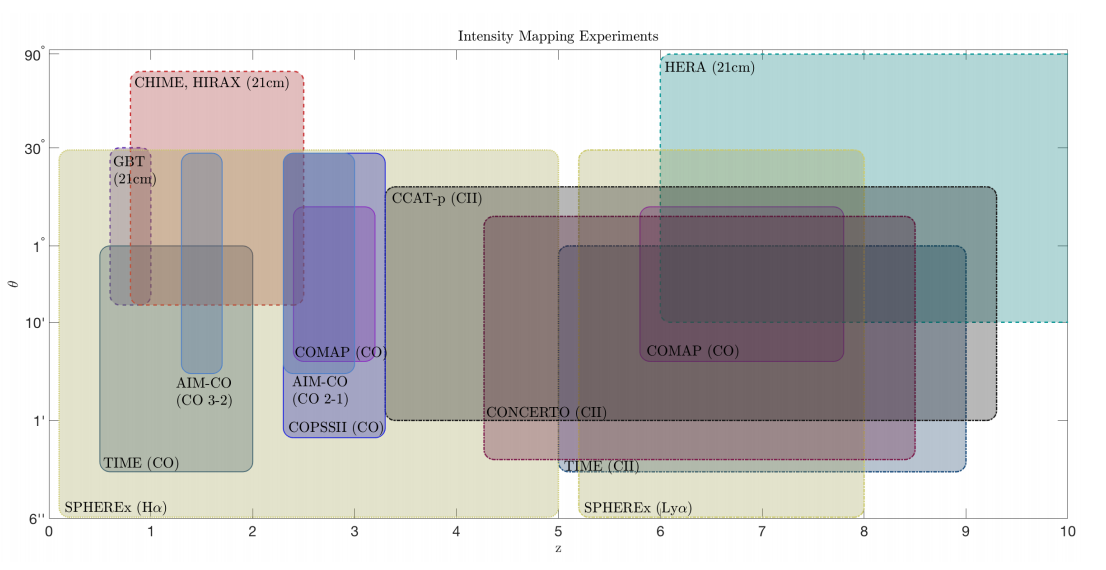
\includegraphics[width=0.95\textwidth]{results/intensity_mapping.png}
	\caption[Resolution and redshift of intensity mapping experiments]{}
	\label{fig:intensity_mapping}
\end{figure}



\tocless\section{\hypertarget{sec:summary}{4.\hspace{0.75em}Summary}}
\addcontentsline{toc}{section}{4.\hspace{0.75em}Summary}

\newpage
\tocless\section{\hypertarget{references}{References}}
\addcontentsline{toc}{section}{References}
\bibliographystyle{aasjournal}
\nocite{*}
\bibliography{refs}

\newpage
\tocless\section{\hypertarget{appendix}{Appendix}}
\addcontentsline{toc}{section}{Appendix}

This is where appendix-y things go


\end{document}
